\documentclass{standalone}

\usepackage{pgfplots,tikz,amsmath}
\begin{document}
        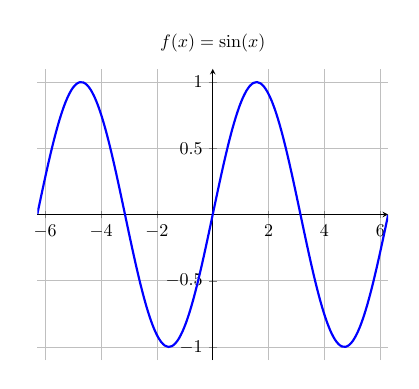
\begin{tikzpicture}[scale=0.65]
            \begin{axis}[axis lines=center, title={$f(x) = \sin(x)$}, domain=-6.28:6.28,
                ymin=-1.1, ymax = 1.1, grid]
                \addplot[smooth, very thick, blue, samples=100] {sin(deg(x))};
            \end{axis}
        \end{tikzpicture}
        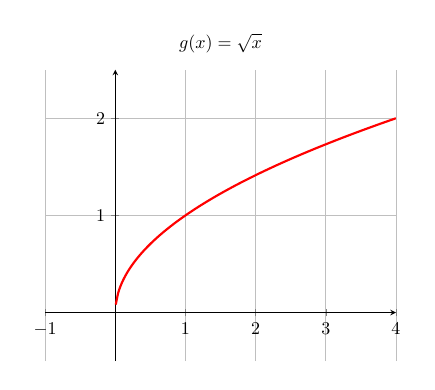
\begin{tikzpicture}[scale=0.65]
            \begin{axis}[axis lines=center, title={$g(x) = \sqrt{x}$}, domain=-1:4,
                ymin=-0.5, ymax = 2.5, xmin=-1, grid]
                \addplot[smooth, very thick, red, samples=150] {sqrt(x)};
            \end{axis}
        \end{tikzpicture}
        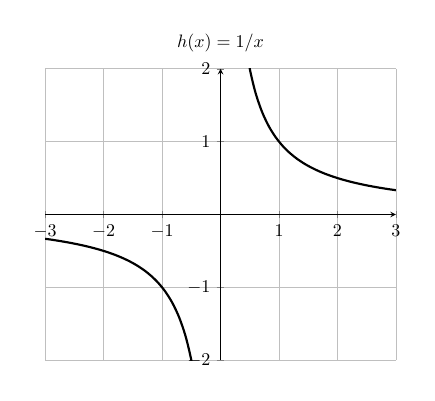
\begin{tikzpicture}[scale=0.65]
            \begin{axis}[axis lines=center, title={$h(x) = 1/x$},
                ymin=-2, ymax = 2, grid]
                \addplot[smooth, very thick, domain=-3:-0.1, black] {1/x};
                \addplot[smooth, very thick, domain=0.1:3, black] {1/x};
            \end{axis}
        \end{tikzpicture}
\end{document}
